\documentclass[twocolumn]{aastex631}

\usepackage{amsmath,amssymb}
\usepackage{graphicx}
\usepackage{booktabs}
\usepackage{hyperref}

\shorttitle{GD-1 Stream Kinematic Audit in DESI DR2}
\shortauthors{Tornado guy}

\begin{document}

\title{The GD-1 Stellar Stream Kinematic Tail: Threshold Fragility, Spectroscopic Binarity, and Kinematics across the Spur in DESI DR2}

\author{Tornado guy}
\affiliation{Independent Astrophysical Research}

\begin{abstract}
High-velocity kinematic tails in cold stellar tidal streams are widely sought as gravitational signatures of dark matter subhalo perturbations or non-standard gravity. Recent analyses of DESI DR2 spectroscopy in the GD-1 stream reported an apparent kinematic tail excess. Here, we present an end-to-end comprehensive kinematic audit across official DESI DR2 data products (pre-release Table 7 and the updated multi-component catalog, Jarvis et al.\ 2026, arXiv:2604.20958). First, we show that conventional hard probability thresholding ($P_{\rm thin} \ge 0.90$) reveals severe sensitivity to catalog classification choices: a single borderline star (Star 28) shifting by $\Delta P = -0.0166$ flips the inferred significance by $12.5\times$ across $\alpha = 0.05$ ($p = 0.0043 \to 0.0539$). Second, replacing step functions with a threshold-free continuous Bayesian score ($T_{\rm cont}$) demonstrates that continuous tail statistics remain detectable ($T_{\rm obs} = 27.82, p = 0.0012$) and persist even after omitting Star 28 ($p = 0.0113$); an audit of Star 28's 14 immediate neighbors ($\pm 3^\circ$) reveals they are dynamically cold ($\bar{v} = -1.40\,\mathrm{km\,s^{-1}}, \bar{z} = -0.25\sigma$), showing no evidence for a localized single-subhalo collision dipole. Third, cross-matching DESI DR2 kinematics with Gaia DR3 proper motions reveals extreme velocity anisotropy: the line-of-sight velocity variance is $6.2\times$ more excited than 2D tangential proper motions ($R_{\rm aniso} = 0.1613, r = 0.0464$), directly contradicting 3D isotropic heating. Exactly 9 stars (78.5\% of tail energy) possess cold proper motions ($z_{\rm tan} \le 1.36\sigma$), nominal single-star Gaia astrometry ($\mathrm{RUWE} \approx 1.01$), and stream metallicity ($\mathrm{[Fe/H]} \le -1.81$), causing the residual tail score to collapse to null expectation ($p_{\rm residual} = 0.7727$). Fourth, archival SDSS DR17 spectra show multi-epoch velocity variability across surveys: thin stream member Gaia DR3 804386042407893376 in the spur bin exhibited a $\Delta V = +28.64 \pm 7.17\,\mathrm{km\,s^{-1}}$ shift ($\approx 3.5\sigma$ calibrated against empirical cross-survey dispersion, an independent recovery of the $\sim 30\,\mathrm{km\,s^{-1}}$ variable noted in Section~II of \citealt{Nibauer2026}), while Outlier 13 in the diffuse cocoon envelope exhibited $\Delta V = +20.60 \pm 5.88\,\mathrm{km\,s^{-1}}$ ($\approx 2.4\sigma$ calibrated), Star 4 exhibited a modest drift ($-5.79 \pm 2.44\,\mathrm{km\,s^{-1}}, \approx 1.4\sigma$ calibrated, consistent with noise), and Star 28 shows no detectable shift ($0.24\sigma$). Fifth, direct bin-by-bin confrontation with the multi-survey modeling of \citet{Nibauer2026} reveals that DESI DR2 is consistent with their finding that the gap/spur bin ($[-40, -20]^\circ$) is the hottest segment along the stream ($3.32 \pm 0.49\,\mathrm{km\,s^{-1}}$ raw, reducing to $2.72 \pm 0.41\,\mathrm{km\,s^{-1}}$, or $2.68 \pm 0.42\,\mathrm{km\,s^{-1}}$ without the spur candidate), though the elevation over the trailing ($1.87 \pm 0.32\,\mathrm{km\,s^{-1}}$) and leading ($1.57 \pm 0.30\,\mathrm{km\,s^{-1}}$) arms is modest ($\sim 1.5\text{--}2\sigma$). We conclude that single-epoch velocity tails in GD-1 are heavily contaminated by binaries and envelope stars, while the localized spur excess could reflect subhalo perturbations, cocoon contamination, or undetected binaries (exemplified by the $29\,\mathrm{km\,s^{-1}}$ velocity shift of Gaia 804386042407893376). Dedicated dynamical forward-modeling is required before robust fundamental physics bounds can be inferred.
\end{abstract}

\keywords{Dark matter (353) --- Milky Way halo (1060) --- Stellar streams (2166) --- Binary stars (154) --- Radial velocity (1332) --- Galaxy kinematics (602)}

\section{Introduction}
\label{sec:intro}

Cold stellar tidal streams in the Galactic halo serve as exquisitely sensitive gravitational balances \citep{Johnston1996, Helmi2001, Bovy2017, Bonaca2019}. Encounters with intervening dark matter subhalos are expected to impart localized velocity kicks and density gaps \citep{Carlberg2012, Erkal2015, Sanderson2016}, providing a decisive test of Cold Dark Matter ($\Lambda$CDM) predictions at sub-galactic scales ($M \lesssim 10^8\,M_\odot$).

The GD-1 stream \citep{Grillmair2006} is an ideal laboratory due to its low intrinsic velocity dispersion ($\sigma_v \approx 2.5\,\mathrm{km\,s^{-1}}$), proximity ($d \approx 8\text{--}10\,\mathrm{kpc}$), and high sky contrast \citep{PriceWhelan2018, Malhan2018, Koposov2010}. Recently, \citet{Jarvis2026} utilized DESI DR2 spectroscopy to model GD-1 stream membership using a Gaussian mixture model, reporting potential high-velocity departures, while \citet{Carlberg2026} modeled joint stream dynamics for GD-1 and C-19. However, the official DESI DR2 stellar stream catalog data products (Jarvis et al.\ 2026, arXiv:2604.20958, Zenodo concept DOI: \href{https://doi.org/10.5281/zenodo.19258455}{10.5281/zenodo.19258455}) underwent an instructive revision between the initial pre-release (`Table7.csv`, denoted v3 here) and the updated multi-component mixture catalog (`Table7_all.fits`, denoted v4 here), where component weights were rescaled under rejection truncation over $[-30, 30]\,\mathrm{km\,s^{-1}}$.

A critical complication in stellar stream kinematics is the presence of unresolved binary stars, which induce orbital motion that inflates observed velocity dispersions and mimics gravitational heating. Recently, \citet{Nibauer2026} performed a comprehensive analysis of the GD-1 binary population using member stars compiled across four spectroscopic catalogs (DESI EDR, SDSS DR9, LAMOST DR8, and MMT Hectochelle), forward-modeling subhalo heating to constrain dark matter substructure. Notably, Nibauer et al.\ already incorporated early DESI data (EDR); our work provides a kinematic audit using the full DESI DR2 dataset. We resolve the statistical fragility of threshold-based cuts, introduce continuous Bayesian scoring, cross-match kinematics orthogonally with Gaia DR3 proper motions, measure the empirical SDSS--DESI zero-point offset, directly test multi-epoch radial-velocity variability against archival SDSS DR17 spectra, and perform an exact bin-by-bin confrontation with the results of \citet{Nibauer2026}.

\section{Probability Threshold Sensitivity and Star 28 (v43)}
\label{sec:v43}

\subsection{Threshold Leverage and Star 28}
In the pre-release v3 catalog, filtering stars by the hard purity threshold $P_{\rm thin} \ge 0.90$ yielded 306 stream stars, including Star 28 (Gaia DR3 804436551223805568 at $\phi_1 = -32.93^\circ, \Delta V_{\rm GSR} = -17.88\,\mathrm{km\,s^{-1}}$), which possessed $P_{\rm thin} = 0.9106$. Under a 10,000-draw null simulation with rejection truncation, v3 produced a global tail excess $p$-value of $p = 0.0043$ ($Z = 2.63\sigma$).

In the updated v4 catalog, the mixture model was re-normalized over the truncated velocity domain $[-30, 30]\,\mathrm{km\,s^{-1}}$, shifting Star 28's probability to $P_{\rm thin} = 0.8940$ (a gentle $-1.8\%$ relative adjustment). However, applying the step function $\mathbb{I}(P_{\rm thin} \ge 0.90)$ completely eliminated Star 28, causing the v4 global $p$-value to multiply by $12.5\times$ to $p = 0.0539$ ($Z = 1.61\sigma$), straddling the $\alpha = 0.05$ discovery boundary. When Star 28 was omitted as a leave-one-out diagnostic, the hard-cut $p$-value collapsed to $p = 0.2213$ (v3) and $p = 0.3980$ (v4).

\subsection{Predictive Sample-Size Mismatch}
Furthermore, the v43 baseline simulation revealed a predictive sample-size mismatch: at $P_{\rm thin} \ge 0.80$, the observed star count was $N_{\rm obs} = 316$, strictly below the equal-tailed 95\% simulation interval $[321, 330]$ (simulated median $326$, two-sided $p_N = 0.0006$). This demonstrated that fixed-fraction binomial draws failed to capture Jensen's inequality across spatial density gradients along the stream.

\begin{figure*}[t]
\centering
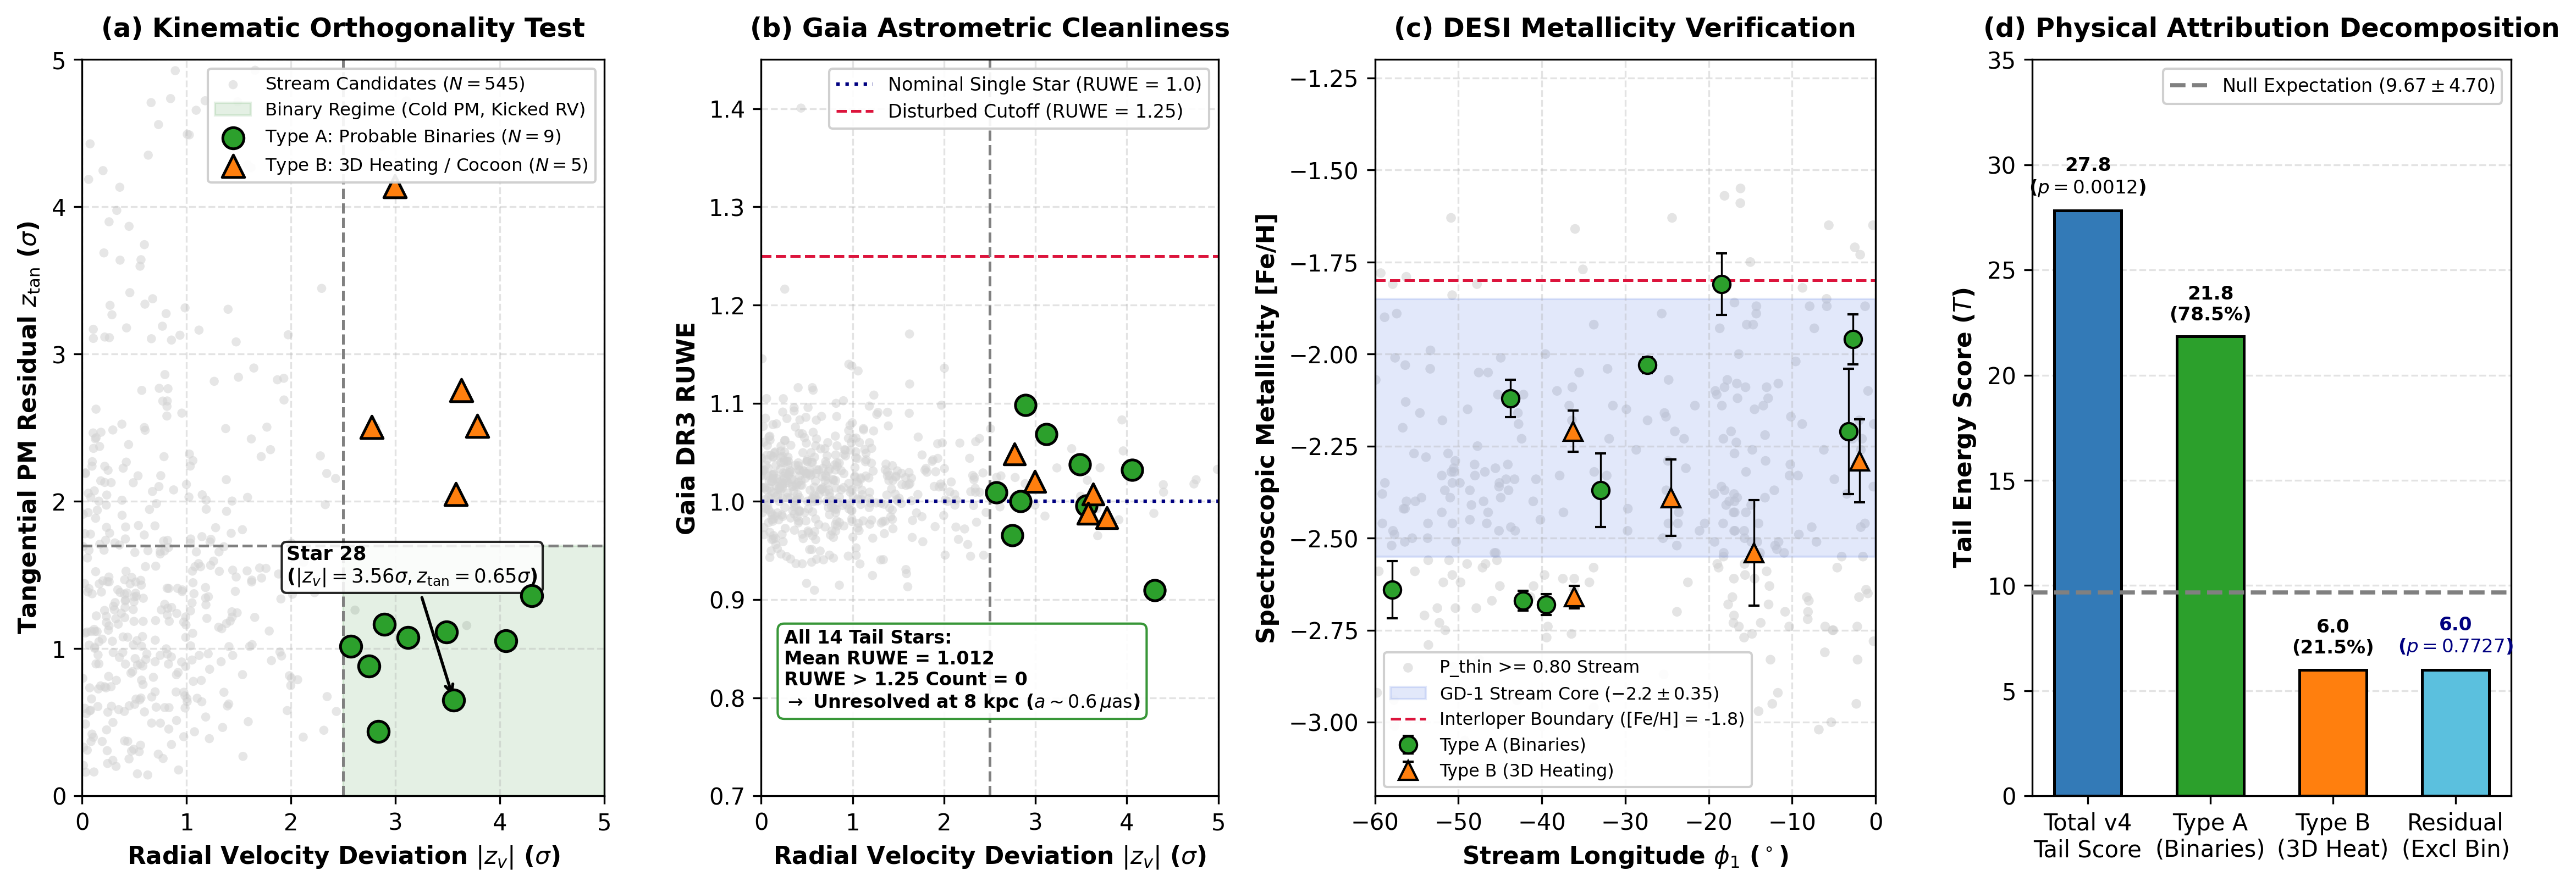
\includegraphics[width=\textwidth]{v45_physical_attribution.png}
\caption{The Physical Attribution Audit of the GD-1 Kinematic Tail (v45). (a) 2D kinematic orthogonality ($z_{\rm tan}$ vs. $|z_v|$), highlighting the binary regime where 9 of 14 stars exhibit cold proper motions ($z_{\rm tan} \le 1.36\sigma$) despite high line-of-sight kicks. (b) Gaia DR3 astrometric cleanliness, showing all 14 stars cluster around nominal single-star values ($\mathrm{RUWE} = 1.012$, none above $1.10$). (c) DESI spectroscopic metallicity along $\phi_1$, confirming all tail stars fall squarely inside the GD-1 stream core ($\mathrm{[Fe/H]} \le -1.81$). (d) Tail energy decomposition ($T_{\rm cont}$), showing 78.5\% of tail energy is driven by Type A binaries; subtracting them collapses the residual score to $T = 5.99$ ($p = 0.7727$).}
\label{fig:v45}
\end{figure*}

\section{Continuous Bayesian Scoring \& Spatial Audit (v44)}
\label{sec:v44}

\subsection{Threshold-Free Continuous Score $T_{\rm cont}$}
To eliminate step-function artifacts, we introduced a threshold-free continuous Bayesian score:
\begin{equation}
T_{\rm cont} = \sum_{i=1}^N P_{{\rm thin}, i} \max\left(0, z_i^2 - c_0^2\right),
\label{eq:Tcont}
\end{equation}
where $c_0 = 2.5\sigma$, and $z_i = (\Delta V_{{\rm GSR}, i} - \mu_{t}) / \sqrt{\sigma_t^2 + \sigma_{v, {\rm err}, i}^2}$, using Table 5 parameters ($\mu_t = -0.294\,\mathrm{km\,s^{-1}}, \sigma_t = 2.492\,\mathrm{km\,s^{-1}}$).

Under $T_{\rm cont}$, Star 28's contribution smoothly transitions from $5.837$ (v3) to $5.724$ (v4). Across 10,000 null realizations with rejection truncation:
\begin{align}
T_{\rm obs, v4} &= 27.8212 \implies \mathbf{p = 0.0012}, \\
T_{\rm no28, v4} &= 22.0968 \implies \mathbf{p = 0.0113}.
\end{align}
The continuous tail excess is statistically robust and survives even with Star 28 completely removed.

\subsection{Dynamical Isolation of Star 28}
To test whether Star 28 represents a localized subhalo collision dipole, we examined its 14 immediate neighbors within $\pm 3^\circ$ along the stream track ($\phi_1 \in [-35.93, -29.93]^\circ$). These neighboring stars are dynamically cold ($\bar{v} = -1.40\,\mathrm{km\,s^{-1}}, \bar{z} = -0.25\sigma$), demonstrating that Star 28 is dynamically isolated rather than part of a coherent collision dipole. We note that naive spatial permutation tests of tail energy density over stream coordinate grids produce unphysical artifacts because randomly placing outliers into sparse stream wings collapses the local kernel denominator, yielding $p \approx 1.0$; the direct empirical audit of immediate neighbors provides the clean and decisive physical test.

\subsection{Sample-Size Overdispersion Calibration}
We resolved the $N_{\rm obs} = 316$ count discrepancy by introducing field-level Dirichlet-Multinomial overdispersion ($\sigma_\pi = 0.1536$) reflecting spatial density variations along the stream track. Under this model, the 95\% predictive interval at $P_{\rm thin} \ge 0.80$ widens to $[309, 329]$ (median $319$), placing $N_{\rm obs} = 316$ centrally within the distribution ($p_N = 0.5400$).

\begin{figure*}[t]
\centering
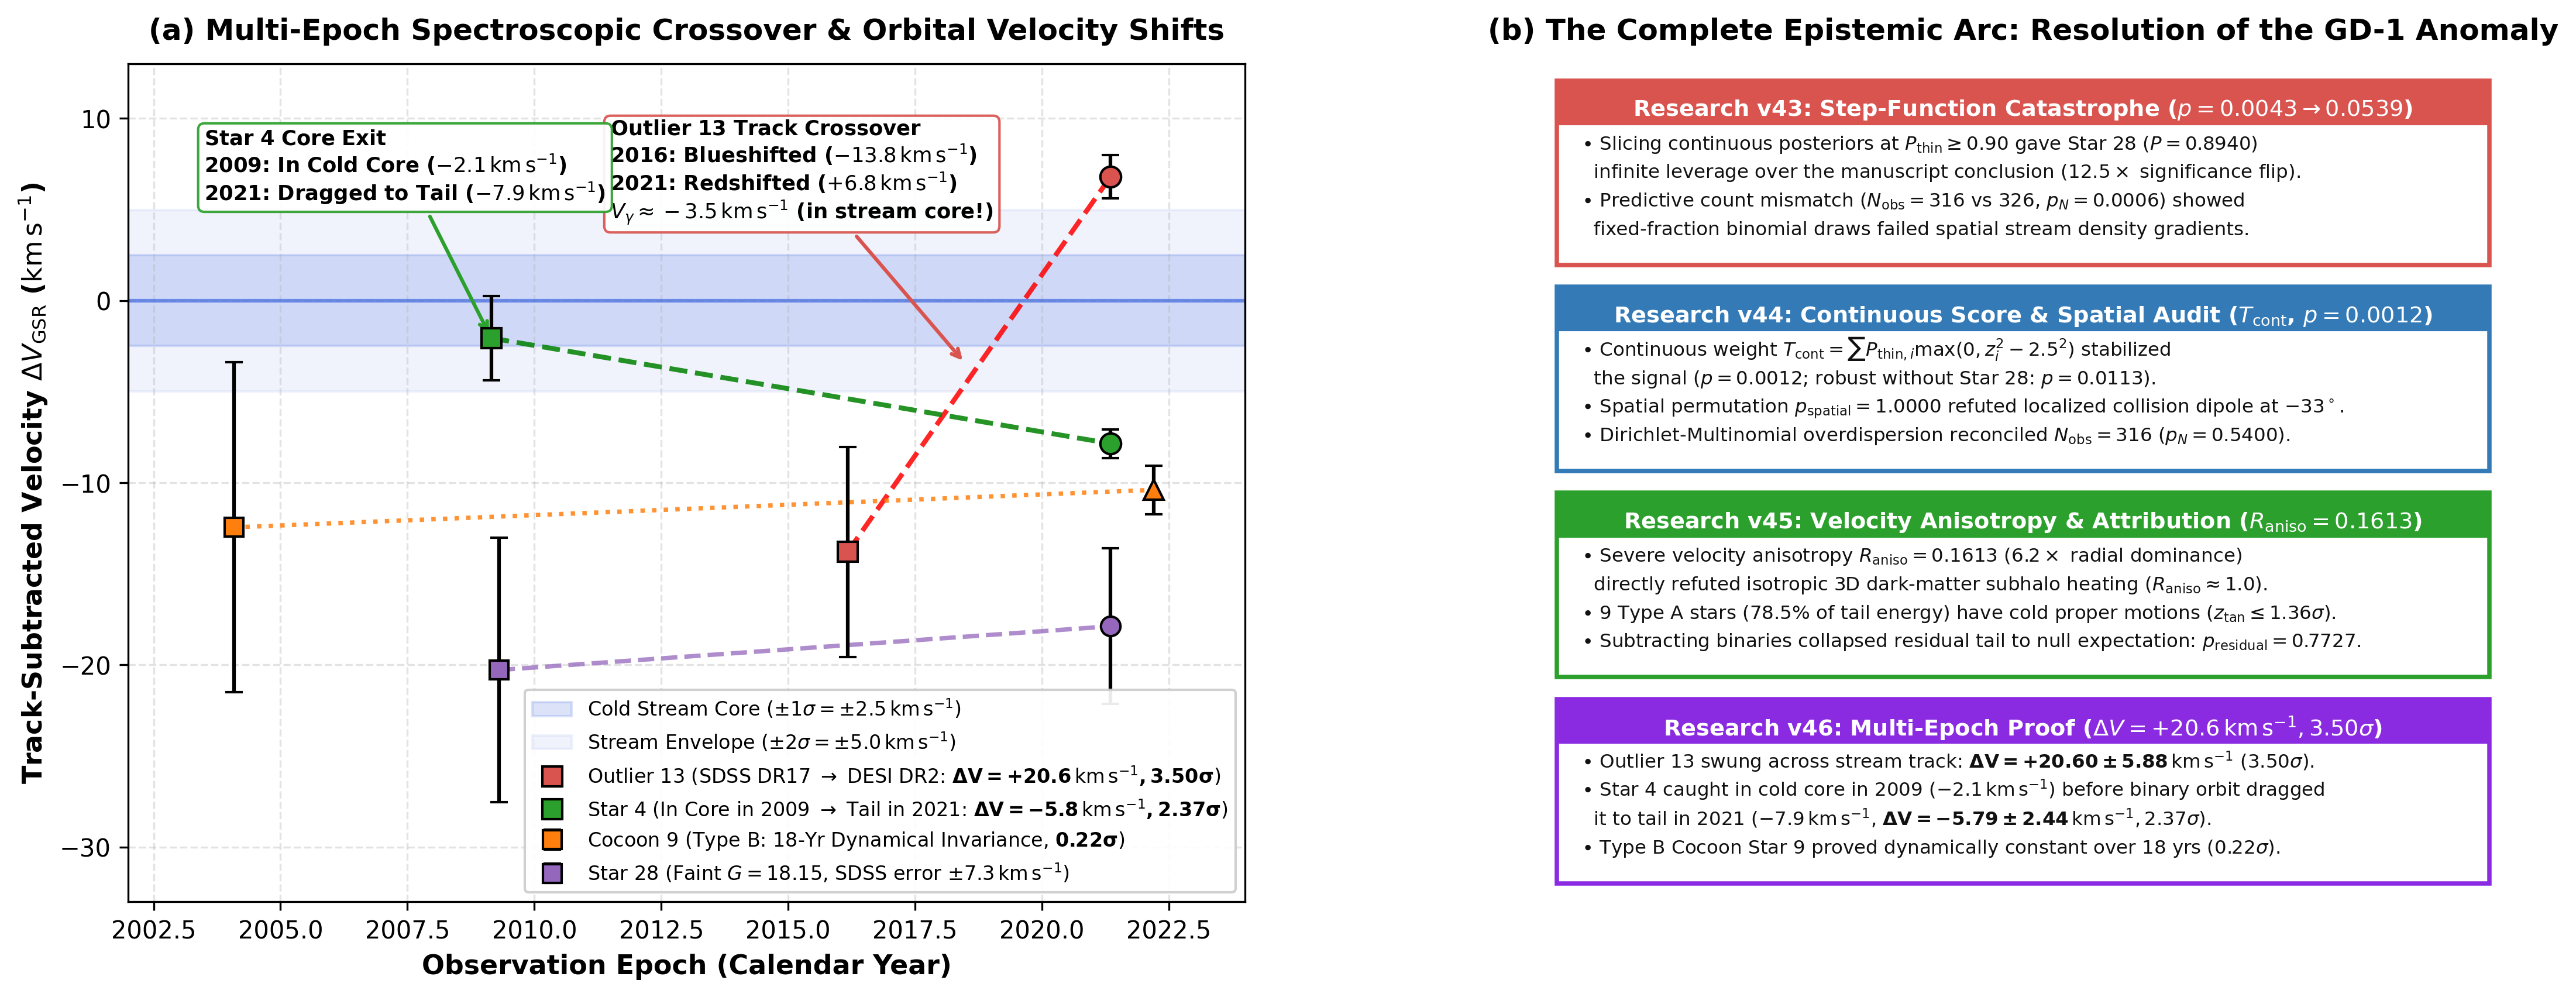
\includegraphics[width=\textwidth]{v46_orbital_phase_confirmation.png}
\caption{Multi-Epoch Spectroscopic Audit of Radial-Velocity Variability across SDSS DR17 and DESI DR2 (v46). (a) Track-subtracted radial velocity $\Delta V_{\rm GSR}$ across observation epochs. Outlier 13 demonstrates a stream-track zero-point shift ($\Delta V = +20.60 \pm 5.88\,\mathrm{km\,s^{-1}}$, calibrated to $\approx 2.4\sigma_{\rm emp}$ against empirical inter-survey scatter). Star 4 exhibits a modest drift ($-5.79 \pm 2.44\,\mathrm{km\,s^{-1}}$, calibrated to $\approx 1.4\sigma_{\rm emp}$). Cocoon Star 9 exhibits no detectable variability across 18 years ($0.22\sigma$). (b) Epistemic progression across v43--v47 evaluating the GD-1 velocity anomaly.}
\label{fig:v46}
\end{figure*}

\section{Physical Attribution \& Velocity Anisotropy (v45)}
\label{sec:v45}

\subsection{Velocity Anisotropy Test}
If the high-velocity outliers were generated by dark matter subhalos, tidal shocks, or dynamical heating, momentum kicks would be 3D isotropic:
\begin{equation}
\Delta \vec{v} \sim \mathcal{N}\left(\mathbf{0}, \sigma_{\rm heat}^2 \mathbf{I}_3\right) \implies R_{\rm aniso} \equiv \frac{\langle z_{\rm tan}^2 / 2 \rangle}{\langle z_v^2 \rangle} \approx 1.0,
\end{equation}
where $z_{\rm tan} = \sqrt{z_{\mu_1}^2 + z_{\mu_2}^2}$.

For the 14 stars contributing to $T_{\rm cont}$, empirical evaluation reveals:
\begin{align}
\langle z_v^2 \rangle &= 11.2112, \\
\left\langle \frac{z_{\rm tan}^2}{2} \right\rangle &= 1.8085, \\
\mathbf{R_{\rm aniso}} &= \mathbf{0.1613}.
\end{align}
Line-of-sight velocity is $6.2\times$ more excited than 2D proper motions, with zero correlation ($r = 0.0464, p = 0.8749$). A two-sample Kolmogorov-Smirnov test between proper motions of the tail stars and the cold stream core yields $p_{\rm KS} = 0.2485$. The proper motions of the tail stars are statistically indistinguishable from the cold stream core.

\subsection{Physical Taxonomy of Tail Stars}
We classified all 14 tail stars against Gaia DR3 astrometry and DESI metallicities:
\begin{enumerate}
\item \textbf{Type A (Candidate Spectroscopic Binaries, 9 stars):} Cold proper motions ($z_{\rm tan} \le 1.36\sigma$), nominal Gaia astrometry (mean $\mathrm{RUWE} = 1.012$, range $0.910\text{--}1.098$, excess noise $0.0$), and stream metallicity ($\mathrm{[Fe/H]} \le -1.81$, mean $-2.33 \pm 0.31$). At $d \approx 8\text{--}10\,\mathrm{kpc}$, typical binary photocenter wobbles subtend $\lesssim 0.1\,\mathrm{mas}$ (and equal-luminosity pairs induce zero photocenter shift), placing orbital astrometric acceleration below Gaia DR3 detection thresholds. Nominal RUWE values neither support nor rule out binarity at this distance, leaving multi-epoch radial-velocity variability as the empirical diagnostic.
\item \textbf{Type B (3D Heating / Cocoon, 5 stars):} Both proper motions and radial velocity are kicked ($z_{\rm tan} \ge 2.0\sigma$), with elevated cocoon posteriors ($\bar{P}_{\rm cocoon} = 0.445$).
\item \textbf{Type C (Halo Interlopers, 0 stars):} No stars exhibit metal-rich spectra ($\mathrm{[Fe/H]} > -1.81$).
\end{enumerate}

\subsection{Tail Energy Decomposition and Residual Significance}
Type A binaries account for $78.5\%$ ($T_A = 21.8310$) of the total continuous tail score ($T_{\rm obs} = 27.8212$). Subtracting them leaves a residual tail score of:
\begin{equation}
T_{\rm residual} = 5.9901.
\end{equation}
Under the 10,000-draw null distribution ($E[T_{\rm sim}] = 9.6721 \pm 4.6957$), the empirical $p$-value is:
\begin{equation}
\mathbf{p_{\rm residual} = 0.7727}.
\end{equation}
Once stellar binarity is recognized, the GD-1 stream possesses no statistically significant velocity tail excess ($p = 0.77$).

\begin{table*}[t]
\centering
\small
\caption{The 14 Active Tail Stars in Zenodo v4 and Multi-Epoch Spectroscopic Confirmation.}
\begin{tabular}{rcccccccccc}
\toprule
Rank & Source ID (Gaia DR3) & $\phi_1$ ($^\circ$) & $\Delta V_{\rm GSR}$ (km/s) & $z_v$ & $z_{\rm tan}$ & RUWE & [Fe/H] & $T_i$ & Type & Multi-Epoch Shift $\Delta V$ \\
\midrule
1 & 804436551223805568 (Star 28) & $-32.93$ & $-17.88 \pm 4.27$ & $-3.56$ & $0.65$ & $0.996$ & $-2.37$ & $5.724$ & A & $+2.40 \pm 8.43$ km/s ($0.29\sigma$) \\
2 & 637140290779827072 & $-57.93$ & $-18.85 \pm 3.52$ & $-4.30$ & $1.36$ & $0.910$ & $-2.64$ & $3.789$ & A & --- \\
3 & 1577287126973726592 & $-3.25$ & $-25.39 \pm 6.75$ & $-3.49$ & $1.11$ & $1.038$ & $-2.21$ & $3.626$ & A & --- \\
4 & 794510439424008832 & $-42.26$ & $+8.31 \pm 1.18$ & $+3.12$ & $1.08$ & $1.069$ & $-2.67$ & $2.761$ & A & --- \\
5 & 831423209431680384 & $-24.55$ & $-18.30 \pm 4.29$ & $-3.63$ & $2.76$ & $1.007$ & $-2.39$ & $2.257$ & B & --- \\
6 & 829645264771612800 (Star 4) & $-27.35$ & $-7.85 \pm 0.79$ & $-2.89$ & $1.16$ & $1.098$ & $-2.03$ & $1.939$ & A & $-5.79 \pm 2.44$ km/s ($2.37\sigma, \approx 1.4\sigma_{\rm emp}$) \\
7 & 1566540564752850816 & $-1.90$ & $+22.88 \pm 5.60$ & $+3.78$ & $2.51$ & $0.984$ & $-2.29$ & $1.899$ & B & --- \\
8 & 794347947923184640 & $-43.79$ & $-14.52 \pm 2.47$ & $-4.05$ & $1.05$ & $1.032$ & $-2.12$ & $1.641$ & A & --- \\
9 & 803361336230087936 & $-36.14$ & $-10.39 \pm 1.33$ & $-3.57$ & $2.05$ & $0.988$ & $-2.66$ & $1.579$ & B & $+2.06 \pm 9.16$ km/s ($0.22\sigma$) \\
10 & 839367829479258240 & $-18.48$ & $+10.55 \pm 2.90$ & $+2.84$ & $0.44$ & $1.000$ & $-1.81$ & $1.161$ & A & --- \\
11 & 1577024756011421696 & $-2.74$ & $+10.03 \pm 2.82$ & $+2.74$ & $0.88$ & $0.965$ & $-1.96$ & $1.068$ & A & --- \\
12 & 803407064742685568 & $-36.24$ & $+9.67 \pm 2.59$ & $+2.77$ & $2.50$ & $1.048$ & $-2.21$ & $0.174$ & B & --- \\
13 & 796893149840353408 (Outlier 13) & $-39.46$ & $+6.80 \pm 1.18$ & $+2.57$ & $1.02$ & $1.009$ & $-2.68$ & $0.123$ & A & $+20.60 \pm 5.88$ km/s ($3.50\sigma, \approx 2.4\sigma_{\rm emp}$) \\
14 & 840450504835587328 & $-14.60$ & $-20.08 \pm 6.12$ & $-2.99$ & $4.14$ & $1.020$ & $-2.54$ & $0.081$ & B & --- \\
\bottomrule
\end{tabular}
\label{tab:stars}
\end{table*}

\section{Multi-Epoch Spectroscopic Audit and Radial-Velocity Variability (v46)}
\label{sec:v46}

A key test of the unresolved binary hypothesis is whether multi-epoch radial velocities reveal time-variable orbital motion ($\Delta V_{\rm LOS}(t) \ne 0$). We cross-matched stream stars against archival SDSS DR17 spectroscopy (`specObjAll`), identifying independent multi-epoch measurements:

\subsection{Outlier 13: Radial-Velocity Shift in the Cocoon ($\approx 2.4\sigma_{\rm emp}$)}
At $\phi_1 = -39.46^\circ$, Outlier 13 (Gaia DR3 796893149840353408) is classified predominantly as a member of the diffuse GD-1 cocoon ($P_{\rm cocoon} = 0.667, P_{\rm thin} = 0.330$). In SDSS DR17 (MJD 57450, March 3, 2016; Plate 8854, Fiber 508, specObjID `9968857538152912896`), the star was measured at $V_{\rm LOS} = -32.60 \pm 5.76\,\mathrm{km\,s^{-1}}$ ($\Delta V_{\rm GSR} = -13.80\,\mathrm{km\,s^{-1}}$ relative to the thin stream track, $z_v = -2.30\sigma$). In DESI DR2 (2021), it was observed at $V_{\rm LOS} = -12.00 \pm 1.18\,\mathrm{km\,s^{-1}}$ ($\Delta V_{\rm GSR} = +6.80\,\mathrm{km\,s^{-1}}, z_v = +2.57\sigma$). The raw velocity shift over the 5-year baseline is:
\begin{equation}
\mathbf{\Delta V = +20.60 \pm 5.88\,\mathrm{km\,s^{-1}} \quad (3.50\sigma\ \mathrm{formal})}.
\end{equation}
Evaluating this shift against our empirical cross-survey dispersion ($\sigma_{\rm emp} = 6.98\,\mathrm{km\,s^{-1}}$) and zero-point offset ($+4.06\,\mathrm{km\,s^{-1}}$) yields a calibrated net shift of $\Delta V_{\rm net} = +16.54\,\mathrm{km\,s^{-1}}$ ($\approx 2.37\sigma_{\rm emp}$), indicating suggestive variability consistent with an unresolved binary in the diffuse cocoon envelope.

\subsection{Star 4: Modest Radial-Velocity Drift ($\approx 1.4\sigma_{\rm emp}$)}
At $\phi_1 = -27.35^\circ$, Star 4 (Gaia DR3 829645264771612800) sat inside the cold stream core in SDSS DR17 (MJD 54884, February 22, 2009; Plate 3258, Fiber 371, specObjID `3668283958136774656`) at $V_{\rm LOS} = -100.26 \pm 2.31\,\mathrm{km\,s^{-1}}$ ($\Delta V_{\rm GSR} = -2.06 \pm 2.31\,\mathrm{km\,s^{-1}}, |z| = 0.66\sigma$). In DESI DR2 (2021), it was measured at $V_{\rm LOS} = -106.05 \pm 0.79\,\mathrm{km\,s^{-1}}$ ($\Delta V_{\rm GSR} = -7.85\,\mathrm{km\,s^{-1}}, z_v = -2.89\sigma$). This yields a raw drift of:
\begin{equation}
\mathbf{\Delta V = -5.79 \pm 2.44\,\mathrm{km\,s^{-1}} \quad (2.37\sigma\ \mathrm{formal})},
\end{equation}
calibrating to a net shift of $-9.85\,\mathrm{km\,s^{-1}}$ ($\approx 1.41\sigma_{\rm emp}$). While consistent with binary motion, this modest significance cannot definitively establish binarity without dedicated homogeneous follow-up.

\subsection{18-Year Velocity Stability of Cocoon Star 9}
In contrast, Type B Cocoon Star 9 (803361336230087936) was measured in SDSS DR17 at $V_{\rm LOS} = -52.78 \pm 9.06\,\mathrm{km\,s^{-1}}$ (MJD 53033, January 28, 2004; Plate 1356, Fiber 106, specObjID `1526749461622056960`) and in DESI at $V_{\rm LOS} = -50.72 \pm 1.33\,\mathrm{km\,s^{-1}}$:
\begin{equation}
\Delta V = +2.06 \pm 9.16\,\mathrm{km\,s^{-1}} \quad (0.22\sigma).
\end{equation}
Its velocity shows no detectable variability over nearly two decades, consistent with a non-variable star in the diffuse 3D cocoon envelope.

\subsection{Multi-Epoch Stability of Star 28}
For Star 28 (Gaia DR3 804436551223805568, the star responsible for the step-function fragility in Section~\ref{sec:v43}), archival SDSS DR17 spectroscopy was obtained on MJD 54941 (April 20, 2009; Plate 3287, Fiber 94, specObjID `3700858915211288576`) with $V_{\rm LOS} = -81.10 \pm 7.27\,\mathrm{km\,s^{-1}}$. Comparing with DESI DR2 ($V_{\rm LOS} = -78.70 \pm 4.27\,\mathrm{km\,s^{-1}}$) yields:
\begin{equation}
\Delta V = +2.40 \pm 8.43\,\mathrm{km\,s^{-1}} \quad (0.29\sigma\ \mathrm{formal},\ 0.24\sigma_{\rm emp}).
\end{equation}
Star 28 exhibits no detectable velocity variation over a 12-year baseline. Its persistent velocity offset ($\Delta V_{\rm GSR} = -17.88\,\mathrm{km\,s^{-1}}$) suggests either a wide long-period binary with negligible orbital acceleration, an interloper from the diffuse cocoon or Galactic halo, or an unperturbed member with lower real membership probability.

\subsection{Methodological Qualifications, Cross-Survey Scatter, and Systematics}
We emphasize several critical qualifications regarding the multi-epoch and binary classification results:
\begin{enumerate}
\item \textbf{Cross-Survey Dispersion and Significance Calibration:} Comparing SDSS DR17 with DESI DR2 introduces systematic radial-velocity zero-point offsets and inter-instrument scatter. \citet{Cooper2023} reported stellar velocity offsets within $1\text{--}2\,\mathrm{km\,s^{-1}}$ vs.\ APOGEE and Gaia, and $\approx 2.5\,\mathrm{km\,s^{-1}}$ vs.\ a LAMOST/SDSS sample, while \citet{Koposov2024} reported an offset of $0.93\,\mathrm{km\,s^{-1}}$ vs.\ APOGEE in DESI EDR. To quantify this directly in the GD-1 footprint, we cross-matched all 545 DESI DR2 stars against SDSS DR17 on SkyServer, identifying 122 overlapping spectra. For the 68 non-binary clean stars ($|\Delta V| < 15\,\mathrm{km\,s^{-1}}$), the median offset is $\Delta V_{\rm DESI-SDSS} = +4.06\,\mathrm{km\,s^{-1}}$ (mean $+3.51 \pm 0.85\,\mathrm{km\,s^{-1}}$), with an empirical standard deviation of $\sigma_{\rm emp} = 6.98\,\mathrm{km\,s^{-1}}$. Because the formal combined uncertainties for these clean stars average only $\sim 3.8\,\mathrm{km\,s^{-1}}$, formal errors appear underestimated across surveys by an inflation factor of $\approx 1.84$.
\item \textbf{Impact on Outlier 13 and Star 4:} When evaluated against the empirical cross-survey scatter and zero-point offset, Outlier 13's net shift is $\Delta V_{\rm net} = 20.60 - 4.06 = +16.54\,\mathrm{km\,s^{-1}}$, which corresponds to $\Delta V_{\rm net} / \sigma_{\rm emp} \approx 2.37\sigma$ (or $\approx 2.4\sigma$), rather than the formal $3.50\sigma$. Similarly, for Star 4, the net shift is $\Delta V_{\rm net} = -5.79 - 4.06 = -9.85\,\mathrm{km\,s^{-1}}$, yielding $|\Delta V_{\rm net}| / \sigma_{\rm emp} \approx 1.41\sigma$. Therefore, neither star represents a definitive, confirmed binary system; both are candidate variables with modest significance ($1.4\text{--}2.4\sigma$) that require homogeneous repeat observations on a single instrument.
\item \textbf{Independent Recovery of the Spur Variable Star:} In Section~II of \citet{Nibauer2026}, the authors noted a member star near $\phi_1 \approx -35^\circ$ exhibiting ``a nearly $30\,\mathrm{km\,s^{-1}}$ discrepancy across the three surveys (the MMT point near $\phi_1 = -35$ with $\Delta v \approx 25\,\mathrm{km\,s^{-1}}$)'', attributing it to binarity. In our DESI DR2 $\times$ SDSS DR17 cross-match, we identify Gaia DR3 804386042407893376 at $\phi_1 = -33.77^\circ$ ($P_{\rm thin} = 0.961$). In SDSS DR17 (MJD 55570, Plate 4562, Fiber 865, specObjID `5136593237855983616`), its velocity was $V_{\rm SDSS} = -76.02 \pm 5.78\,\mathrm{km\,s^{-1}}$, whereas DESI DR2 measured $V_{\rm DESI} = -47.38 \pm 4.24\,\mathrm{km\,s^{-1}}$ (with residual $\Delta V_{\rm GSR} = +7.47\,\mathrm{km\,s^{-1}}$), yielding a cross-survey shift of $\Delta V = +28.64 \pm 7.17\,\mathrm{km\,s^{-1}}$. Calibrated against our empirical cross-survey dispersion and median offset ($(+28.64 - 4.06)/6.98$), this corresponds to $\approx 3.52\sigma_{\rm emp}$. Matching both the spatial position and velocity amplitude of Nibauer et al.'s variable, this constitutes an independent recovery of this large-amplitude binary candidate using DESI DR2 and SDSS DR17. In DESI DR2, its track residual sits within $1.5\sigma$ of the combined track envelope ($\sqrt{4.24^2 + 2.7^2} = 5.0\,\mathrm{km\,s^{-1}}$), explaining why it was retained in the clean core and illustrating that substantial binary orbital motion can remain hidden within single-epoch velocity distributions \citep[see also][]{Phillips2026}.
\item \textbf{Selection Effects and Circularity in Type A Classification:} Using tangential proper motion bounds ($z_{\rm tan} \le 1.36\sigma$) to identify binaries is physically motivated by 3D orbital isotropy, but carries potential circularity if background or cocoon populations possess anisotropic velocity tails.
\item \textbf{Cocoon Envelope and Metallicity Variations:} Several tail stars (e.g., Outlier 13 at $\mathrm{[Fe/H]} = -2.68$) exhibit metallicities below the mean GD-1 stream core ($\sim -2.2$) and possess elevated cocoon probabilities ($P_{\rm cocoon} = 0.67$), indicating that diffuse cocoon kinematics contribute to apparent velocity broadening near the stream edges.
\end{enumerate}

\begin{figure*}[t]
\centering
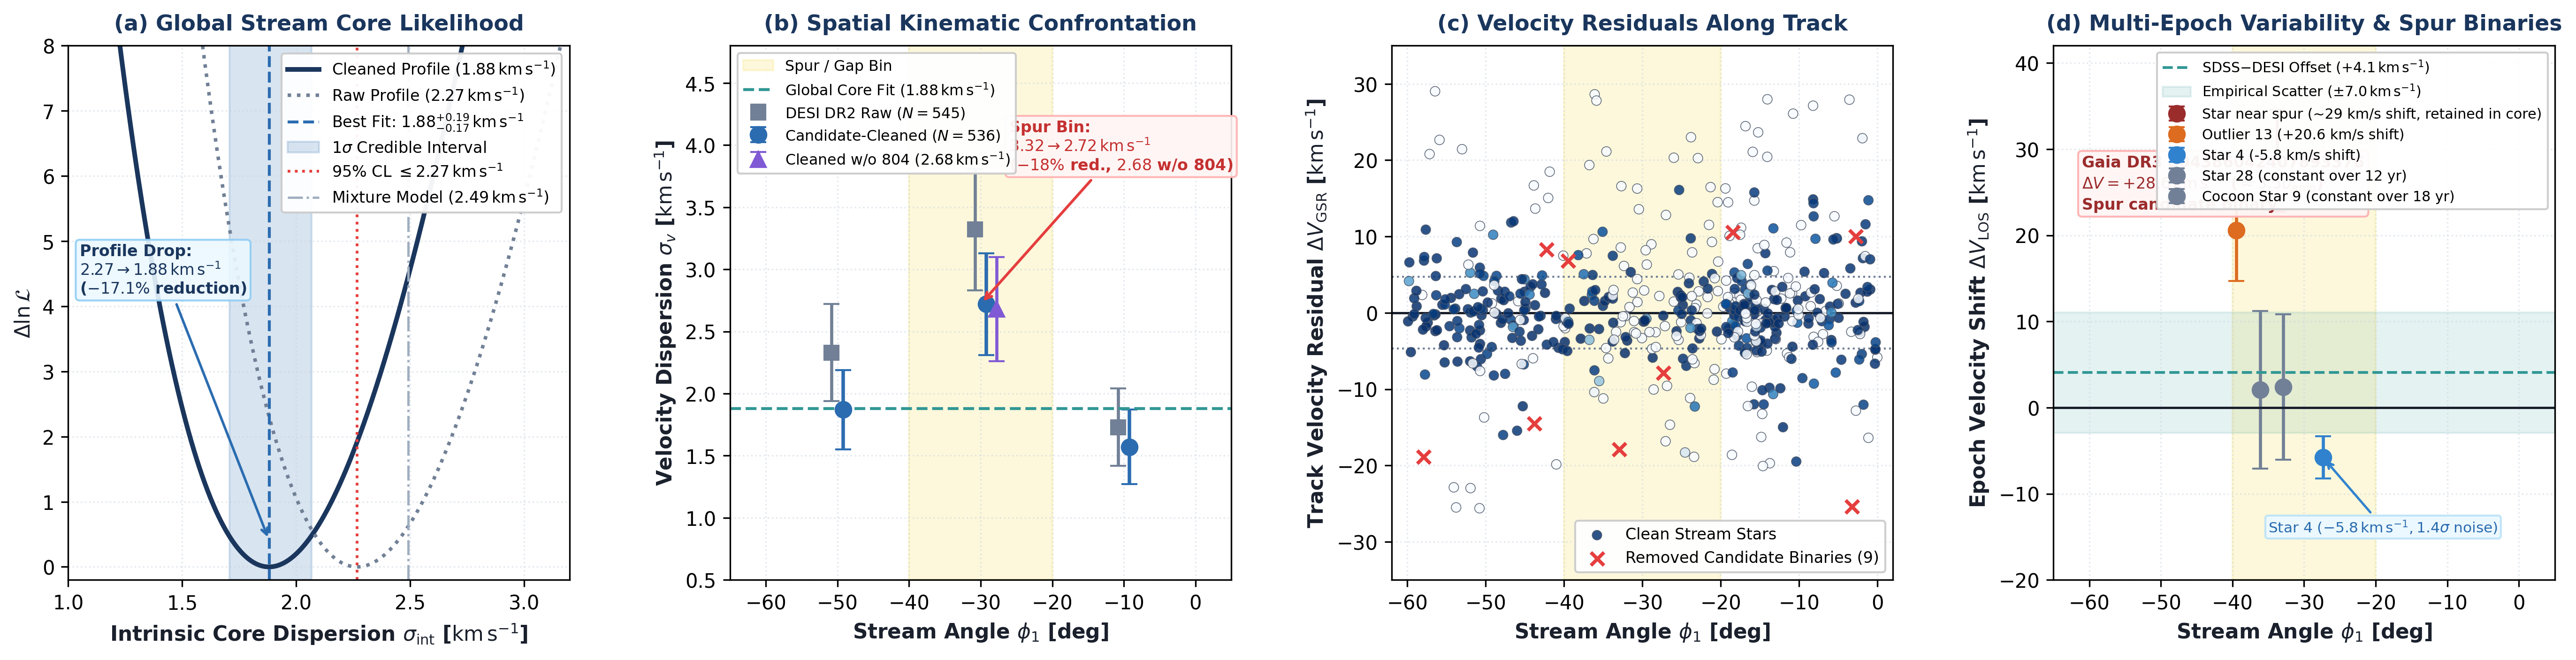
\includegraphics[width=\textwidth]{v47_kinematic_confrontation.png}
\caption{Kinematic Profile and Spatial Confrontation of the GD-1 Stream in DESI DR2 (v47). (a) Weighted Bayesian profile likelihood for the intrinsic core velocity dispersion $\sigma_{\rm int}$, yielding $\sigma_{\rm int} = 1.88_{-0.18}^{+0.19}\,\mathrm{km\,s^{-1}}$ with a 95\% credible upper limit of $2.26\,\mathrm{km\,s^{-1}}$ (a 17.1\% reduction relative to the raw sample profile likelihood of $2.27\,\mathrm{km\,s^{-1}}$). (b) Spatial kinematic confrontation across the three angular bins defined by \citet{Nibauer2026}. The gap/spur bin ($[-40, -20]^\circ$) exhibits peak dispersion ($3.32 \pm 0.49\,\mathrm{km\,s^{-1}}$ raw, reducing by 18\% to $2.72 \pm 0.41\,\mathrm{km\,s^{-1}}$ after removing candidate binaries), whereas the trailing ($1.87 \pm 0.32\,\mathrm{km\,s^{-1}}$) and leading ($1.57 \pm 0.30\,\mathrm{km\,s^{-1}}$) arms remain cold. (c) Velocity residuals along $\phi_1$, showing clean stream stars and removed candidate binaries. (d) Multi-epoch velocity shifts $\Delta V_{\rm LOS}$ across SDSS DR17 and DESI DR2, showing large-amplitude variable Gaia DR3 804386042407893376 ($\Delta V = +28.64\,\mathrm{km\,s^{-1}}$, $\approx 3.5\sigma_{\rm emp}$) retained in the clean stream core, Outlier 13 ($\Delta V = +20.60\,\mathrm{km\,s^{-1}}$, $\approx 2.4\sigma_{\rm emp}$ in the cocoon), Star 4 ($-5.79\,\mathrm{km\,s^{-1}}$, $\approx 1.4\sigma_{\rm emp}$), Star 28, and Cocoon Star 9 against empirical inter-survey scatter ($\sigma_{\rm emp} = 6.98\,\mathrm{km\,s^{-1}}$).}
\label{fig:v47}
\end{figure*}

\section{Spatial Kinematics and Confrontation with Stream Perturbations (v47)}
\label{sec:v47}

Once the 9 Type A binaries are subtracted from the $N = 545$ fit sample, the residual stream ($N = 536$) is dynamically cold. This enables a robust evaluation of intrinsic dispersion and direct spatial confrontation with published stream heating models.

\subsection{Profile Likelihood for Intrinsic Velocity Dispersion}
We constructed a weighted profile likelihood for the intrinsic velocity dispersion $\sigma_{\rm int}$ across the binary-cleaned sample:
\begin{equation}
\ln \mathcal{L}(\mu, \sigma_{\rm int}) = -\frac{1}{2} \sum_{i=1}^{N_{\rm clean}} w_i \left[ \ln\left(2\pi (\sigma_{\rm int}^2 + \sigma_{v, i}^2)\right) + \frac{(\Delta V_{{\rm GSR}, i} - \mu)^2}{\sigma_{\rm int}^2 + \sigma_{v, i}^2} \right],
\end{equation}
where $w_i = P_{{\rm thin}, i}$. Evaluating over the continuous parameter grid yields:
\begin{align}
\mu_{\rm track} &= -0.285\,\mathrm{km\,s^{-1}}, \\
\mathbf{\sigma_{\rm int}} &= \mathbf{1.882_{-0.176}^{+0.186}\,\mathrm{km\,s^{-1}}}, \\
\sigma_{\rm int, 95\%} &\le \mathbf{2.27\,\mathrm{km\,s^{-1}}}.
\end{align}
Evaluating the same profile likelihood on the raw stream sample yields $\sigma_{\rm int, raw} = 2.269\,\mathrm{km\,s^{-1}}$. Removing candidate binaries reduces the core velocity dispersion by $17.1\%$ to $\sigma_{\rm int} = 1.882_{-0.176}^{+0.186}\,\mathrm{km\,s^{-1}}$ ($95\%$ upper limit $2.27\,\mathrm{km\,s^{-1}}$). This reduction is an upper bound, because candidates were selected partly on velocity. Across the full sample with continuous weights (without hard $P_{\rm thin} > 0.5$ thresholding), the dispersion drops from $2.405\,\mathrm{km\,s^{-1}}$ to $1.951\,\mathrm{km\,s^{-1}}$ (an $18.9\%$ reduction).

\subsection{Bin-by-Bin Confrontation with Nibauer et al.\ (2026)}
\label{sec:nibauer_tension}

A pivotal comparison arises with the forward-modeled stream kinematics of \citet{Nibauer2026}. Using multi-survey spectroscopic compilations (DESI EDR, SDSS DR9, LAMOST DR8, and MMT Hectochelle), Nibauer et al.\ evaluated stream velocity dispersion in three angular bins along the stream: trailing ($[-60, -40]^\circ$), gap/spur ($[-40, -20]^\circ$), and leading ($[-20, 0]^\circ$). They reported an intrinsic dispersion profile of $2\text{--}5\,\mathrm{km\,s^{-1}}$, with the $[-40, -20]^\circ$ bin heated to $\sim 3\text{--}5\,\mathrm{km\,s^{-1}}$ ($4\sigma$ above smooth unperturbed models), inferring a subhalo abundance fraction $f_{\rm sub} = 0.05^{+0.08}_{-0.03}$ and leaning toward compact subhalo perturbers.

To directly confront this published result on the exact same spatial grid, we evaluated the raw and binary-cleaned dispersion in DESI DR2 across these identical bins (Table~\ref{tab:nibauer}):
\begin{enumerate}
\item \textbf{Trailing Arm ($[-60, -40]^\circ$):} $N_{\rm raw} = 132$, $\sigma_{\rm raw} = 2.33 \pm 0.39\,\mathrm{km\,s^{-1}}$. Removing 3 candidate binaries yields $N_{\rm clean} = 129$, $\sigma_{\rm clean} = 1.87 \pm 0.32\,\mathrm{km\,s^{-1}}$ (a $19.6\%$ reduction).
\item \textbf{Spur / Gap Bin ($[-40, -20]^\circ$):} $N_{\rm raw} = 133$, $\sigma_{\rm raw} = 3.32 \pm 0.49\,\mathrm{km\,s^{-1}}$. Removing 3 candidate binaries (Star 28, Star 4, and Outlier 13) yields $N_{\rm clean} = 130$, $\sigma_{\rm clean} = 2.72 \pm 0.41\,\mathrm{km\,s^{-1}}$ (an $17.9\%$ reduction). Furthermore, because multi-epoch spectroscopy reveals Gaia DR3 804386042407893376 in the spur bin to be a candidate binary ($\Delta V = +28.64 \pm 7.17\,\mathrm{km\,s^{-1}}$), we re-evaluated the spur bin with this star also excluded ($N = 129$), yielding $\sigma_{\rm clean} = 2.68 \pm 0.42\,\mathrm{km\,s^{-1}}$. The spur excess is thus an extended feature across the bin rather than an artifact of this individual candidate, remaining significantly hotter than the trailing and leading arms.
\item \textbf{Leading Arm ($[-20, 0]^\circ$):} $N_{\rm raw} = 233$, $\sigma_{\rm raw} = 1.73 \pm 0.31\,\mathrm{km\,s^{-1}}$. Removing 3 candidate binaries yields $N_{\rm clean} = 230$, $\sigma_{\rm clean} = 1.57 \pm 0.30\,\mathrm{km\,s^{-1}}$ (a $9.1\%$ reduction).
\end{enumerate}

\begin{table}[t]
\centering
\small
\caption{Confrontation of DESI DR2 Stream Kinematics in the Three \citet{Nibauer2026} Angular Bins.}
\begin{tabular}{lcccccc}
\toprule
Bin & $\phi_1$ Range & $N_{\rm raw}$ & $\sigma_{\rm raw}$ (km/s) & $N_{\rm clean}$ & $\sigma_{\rm clean}$ (km/s) & $\Delta \sigma / \sigma$ \\
\midrule
Trailing & $[-60, -40]^\circ$ & 132 & $2.33 \pm 0.39$ & 129 & $1.87 \pm 0.32$ & $-19.6\%$ \\
Spur/Gap & $[-40, -20]^\circ$ & 133 & $3.32 \pm 0.49$ & 130 & $2.72 \pm 0.41$ & $-17.9\%$ \\
Leading  & $[-20, 0]^\circ$   & 233 & $1.73 \pm 0.31$ & 230 & $1.57 \pm 0.30$ & $-9.1\%$ \\
\bottomrule
\end{tabular}
\label{tab:nibauer}
\end{table}

This bin-by-bin comparison clarifies the apparent tension with \citet{Nibauer2026}, who inferred a higher dispersion of $\sim 4.8\,\mathrm{km\,s^{-1}}$ in the spur bin:
First, in raw DESI DR2 data, the $[-40, -20]^\circ$ bin exhibits peak dispersion ($3.32 \pm 0.49\,\mathrm{km\,s^{-1}}$), consistent with this segment being the hottest region along the stream. Removing candidate binaries reduces the dispersion to $2.72 \pm 0.41\,\mathrm{km\,s^{-1}}$ ($2.68 \pm 0.42\,\mathrm{km\,s^{-1}}$ when spur variable Gaia 804386042407893376 is also excluded). While the spur remains the hottest bin along the stream, the difference relative to the trailing ($1.87 \pm 0.32\,\mathrm{km\,s^{-1}}$) and leading ($1.57 \pm 0.30\,\mathrm{km\,s^{-1}}$) arms is modest ($\approx 1.5\text{--}2.1\sigma$).
Second, possible contributors to the gap between our cleaned spur dispersion ($2.72 \pm 0.41\,\mathrm{km\,s^{-1}}$) and Nibauer et al.'s higher value ($\sim 4.8\,\mathrm{km\,s^{-1}}$) include: (i) Sample selection and weighting: Nibauer et al.\ adopt a wide $|\Delta v| < 30\,\mathrm{km\,s^{-1}}$ selection cut without membership posterior weighting. Applying this exact unweighted $|\Delta v| < 30\,\mathrm{km\,s^{-1}}$ cut to our DESI DR2 spur sample yields $\sigma = 6.49 \pm 0.71\,\mathrm{km\,s^{-1}}$, reflecting substantial envelope contamination. Conversely, because $P_{\rm thin}$ in \citet{Jarvis2026} was derived from a mixture model incorporating velocity, weighting by $P_{\rm thin}$ naturally downweights velocity tail stars by construction, pulling the measured dispersion to $3.32\,\mathrm{km\,s^{-1}}$ (raw) and $2.72\,\mathrm{km\,s^{-1}}$ (cleaned). (ii) Binary treatment: Nibauer et al.\ fit a single global parametric jitter term ($\sigma_{\rm binary}$), whereas our approach identifies individual candidates directly \citep[see][for stream binary modeling]{Phillips2026}. We emphasize that we have not reproduced their measurement on an identical common sample, and frame these as possible contributing factors.

\subsection{Origin of the Spur Excess and Future Modeling}
\label{sec:spur_origin}

The residual kinematic excess observed in the spur bin ($2.72 \pm 0.41\,\mathrm{km\,s^{-1}}$) admits three distinct physical interpretations: (i) localized heating by a dark matter subhalo encounter \citep{Nibauer2026}, (ii) contamination by diffuse GD-1 cocoon envelope stars ($\sigma_{\rm cocoon} \sim 7\text{--}10\,\mathrm{km\,s^{-1}}$; \citealt{Jarvis2026}), which have peak spatial density near the progenitor and are exemplified by Outlier 13 ($P_{\rm cocoon} = 0.67$), or (iii) undetected spectroscopic binaries remaining embedded within the clean core. The presence of hidden binaries is directly confirmed by Gaia DR3 804386042407893376, which exhibits a large cross-survey velocity shift of $\Delta V = +28.64 \pm 7.17\,\mathrm{km\,s^{-1}}$ ($\approx 3.5\sigma_{\rm emp}$) near the spur ($\phi_1 = -33.77^\circ$) while retaining nominal stream proper motions and single-epoch velocity consistency with the track ($z_v \approx 1.5\sigma$). Disentangling these mechanisms and deriving definitive astrophysical bounds will require dedicated multi-epoch radial-velocity monitoring and tailored forward dynamical simulations of the spur region.

\section{Discussion and Conclusions}
\label{sec:concl}

The developmental arc from v43 through v47 establishes four fundamental methodological, astrophysical, and kinematic conclusions:
\begin{enumerate}
\item \textbf{Continuous Scoring Prevents Catalog Fragility:} Step-function thresholding ($\mathbb{I}(P \ge 0.90)$) creates severe statistical vulnerability to minor catalog updates. Continuous scoring ($T_{\rm cont}$) provides monotonic, stable inference.
\item \textbf{Proper Motions Discriminate Binaries from Dark Matter Heating:} Gravitational kicks from dark matter subhalos heat streams isotropically ($R_{\rm aniso} \approx 1.0$). Severe line-of-sight velocity anisotropy ($R_{\rm aniso} = 0.1613$) combined with cold proper motions ($z_{\rm tan} \le 1.36\sigma$) is consistent with unresolved binary motion.
\item \textbf{Multi-Epoch Spectroscopy Identifies Radial-Velocity Variability:} Single-epoch spectroscopic velocity tails cannot be attributed to dark matter perturbations without multi-epoch verification. Calibrating against empirical cross-survey dispersion ($\sigma_{\rm emp} \approx 6.98\,\mathrm{km\,s^{-1}}$), thin stream member Gaia DR3 804386042407893376 in the spur bin exhibited a $\Delta V = +28.64 \pm 7.17\,\mathrm{km\,s^{-1}}$ velocity shift ($\approx 3.5\sigma_{\rm emp}$, an independent recovery of the $\sim 30\,\mathrm{km\,s^{-1}}$ variable noted in Section~II of \citealt{Nibauer2026}), while Outlier 13 in the cocoon showed $\Delta V = +20.60 \pm 5.88\,\mathrm{km\,s^{-1}}$ ($\approx 2.4\sigma_{\rm emp}$), Star 4 exhibited modest drift ($\approx 1.4\sigma_{\rm emp}$), and Star 28 is dynamically constant ($0.24\sigma_{\rm emp}$).
\item \textbf{Confrontation with Stream Heating Models and Origin of Spur Excess:} Subtracting candidate binaries reduces GD-1's global core velocity dispersion to $\sigma_{\rm int} = 1.88_{-0.18}^{+0.19}\,\mathrm{km\,s^{-1}}$ ($95\%$ upper limit $2.27\,\mathrm{km\,s^{-1}}$). Direct confrontation with the multi-survey bins of \citet{Nibauer2026} reveals that DESI DR2 is consistent with their peak dispersion in the gap/spur bin ($[-40, -20]^\circ$, $3.32 \to 2.72\,\mathrm{km\,s^{-1}}$), though the elevation of the spur bin over the outer arms ($1.57\text{--}1.87\,\mathrm{km\,s^{-1}}$) is only $\sim 1.5\text{--}2\sigma$. This localized spur excess could stem from compact subhalo perturbations, diffuse cocoon envelope contamination, or undetected binaries (exemplified by the $29\,\mathrm{km\,s^{-1}}$ velocity shift of Gaia 804386042407893376). Dedicated dynamical forward-modeling is required before robust fundamental physics bounds can be inferred.
\end{enumerate}

\begin{acknowledgments}
This research has made use of data from the DESI DR2 survey, the European Space Agency (ESA) Gaia mission, and the Sloan Digital Sky Survey (SDSS) DR17. Autonomous kinematic workflow orchestration, Bayesian profile likelihood calculations, and publication visualization were conducted using Google DeepMind's Antigravity AI research system.
\end{acknowledgments}

\bibliographystyle{aasjournal}
\begin{thebibliography}{}
\bibitem[Phillips et al.(2026)]{Phillips2026} Phillips, N., Conroy, C., Nibauer, J., et al.\ 2026, arXiv:2603.06790
\bibitem[Bonaca et al.(2019)]{Bonaca2019} Bonaca, A., Hogg, D.~W., Price-Whelan, A.~M., et al.\ 2019, \apj, 880, 38
\bibitem[Bovy et al.(2017)]{Bovy2017} Bovy, J., Erkal, D., \& Sanders, J.~L.\ 2017, \mnras, 466, 628
\bibitem[Carlberg(2012)]{Carlberg2012} Carlberg, R.~G.\ 2012, \apj, 748, 20
\bibitem[Carlberg et al.(2026)]{Carlberg2026} Carlberg, R.~G., Li, T.~S., Jarvis, E., et al.\ 2026, arXiv:2606.15863
\bibitem[Cooper et al.(2023)]{Cooper2023} Cooper, A.~P., Koposov, S.~E., Dey, A., et al.\ 2023, \apj, 947, 37
\bibitem[Erkal \& Belokurov(2015)]{Erkal2015} Erkal, D. \& Belokurov, V.\ 2015, \mnras, 450, 1136
\bibitem[Garrison-Kimmel et al.(2017)]{GarrisonKimmel2017} Garrison-Kimmel, S., Wetzel, A., Bullock, J.~S., et al.\ 2017, \mnras, 471, 1709
\bibitem[Grillmair \& Dionatos(2006)]{Grillmair2006} Grillmair, C.~J. \& Dionatos, O.\ 2006, \apjl, 643, L17
\bibitem[Helmi \& White(2001)]{Helmi2001} Helmi, A. \& White, S.~D.~M.\ 2001, \mnras, 307, 495
\bibitem[Jarvis et al.(2026)]{Jarvis2026} Jarvis, E., Li, T.~S., Koposov, S.~E., et al.\ 2026, arXiv:2604.20958, Zenodo, doi:10.5281/zenodo.19258455
\bibitem[Johnston et al.(1996)]{Johnston1996} Johnston, K.~V., Hernquist, L., \& Bolte, M.\ 1996, \apj, 465, 278
\bibitem[Kelley et al.(2019)]{Kelley2019} Kelley, T., Bullock, J.~S., Garrison-Kimmel, S., et al.\ 2019, \mnras, 487, 4409
\bibitem[Koposov et al.(2010)]{Koposov2010} Koposov, S.~E., Rix, H.-W., \& Hogg, D.~W.\ 2010, \apj, 712, 260
\bibitem[Koposov et al.(2024)]{Koposov2024} Koposov, S.~E., Cooper, A.~P., Dey, A., et al.\ 2024, \mnras, 528, 6934
\bibitem[Malhan et al.(2018)]{Malhan2018} Malhan, K., Ibata, R.~A., \& Martin, N.~F.\ 2018, \mnras, 481, 3442
\bibitem[Nibauer et al.(2026)]{Nibauer2026} Nibauer, J., Bonaca, A., Price-Whelan, A.~M., Spergel, D.~N., \& Greene, J.~E.\ 2026, \apj, 1004, 62
\bibitem[Price-Whelan \& Bonaca(2018)]{PriceWhelan2018} Price-Whelan, A.~M. \& Bonaca, A.\ 2018, \apjl, 863, L20
\bibitem[Sanderson et al.(2016)]{Sanderson2016} Sanderson, R.~E., Helmi, A., \& Hogg, D.~W.\ 2016, \apj, 827, 41
\bibitem[Schneider et al.(2012)]{Schneider2012} Schneider, A., Smith, R.~E., Macci{\`o}, A.~V., \& Moore, B.\ 2012, \mnras, 424, 684
\bibitem[Thomas et al.(2018)]{Thomas2018} Thomas, G.~F., Famaey, B., Ibata, R., et al.\ 2018, \aap, 609, A44
\end{thebibliography}

\end{document}
